%\lipsum[4-4]
In this chapter is presented the development of the wireless monitoring system, following the specifications and requirements raised in the chapter 2. This chapter is divided in four parts, starting with the description of the selected wireless technology. In \ref{sec:3.3} is presented the hardware and software architecture of the system. Communication results and KPI metrics are presented in section \ref{sec:3.3}. In section \ref{sec:3.4} is made the discussion of the results.

\section{Description of the selected wireless technology}
\label{sec:3.1}
%\lipsum[4-4]

The CC1350 platform was selected to fulfil the wireless requirements. The availability of Sub-1 GHz and Bluetooth technologies in the same device allows enough flexibility in terms of possible functionalities to be implemented. The powerful 32-bit ARM Cortex-M3 allows the implementation of a Real-time Operating System, capable of handling several tasks.

\section{Hardware and software architecture}
\label{sec:3.2}
%\lipsum[4-4]


\begin{figure}[h!]
	\centering
	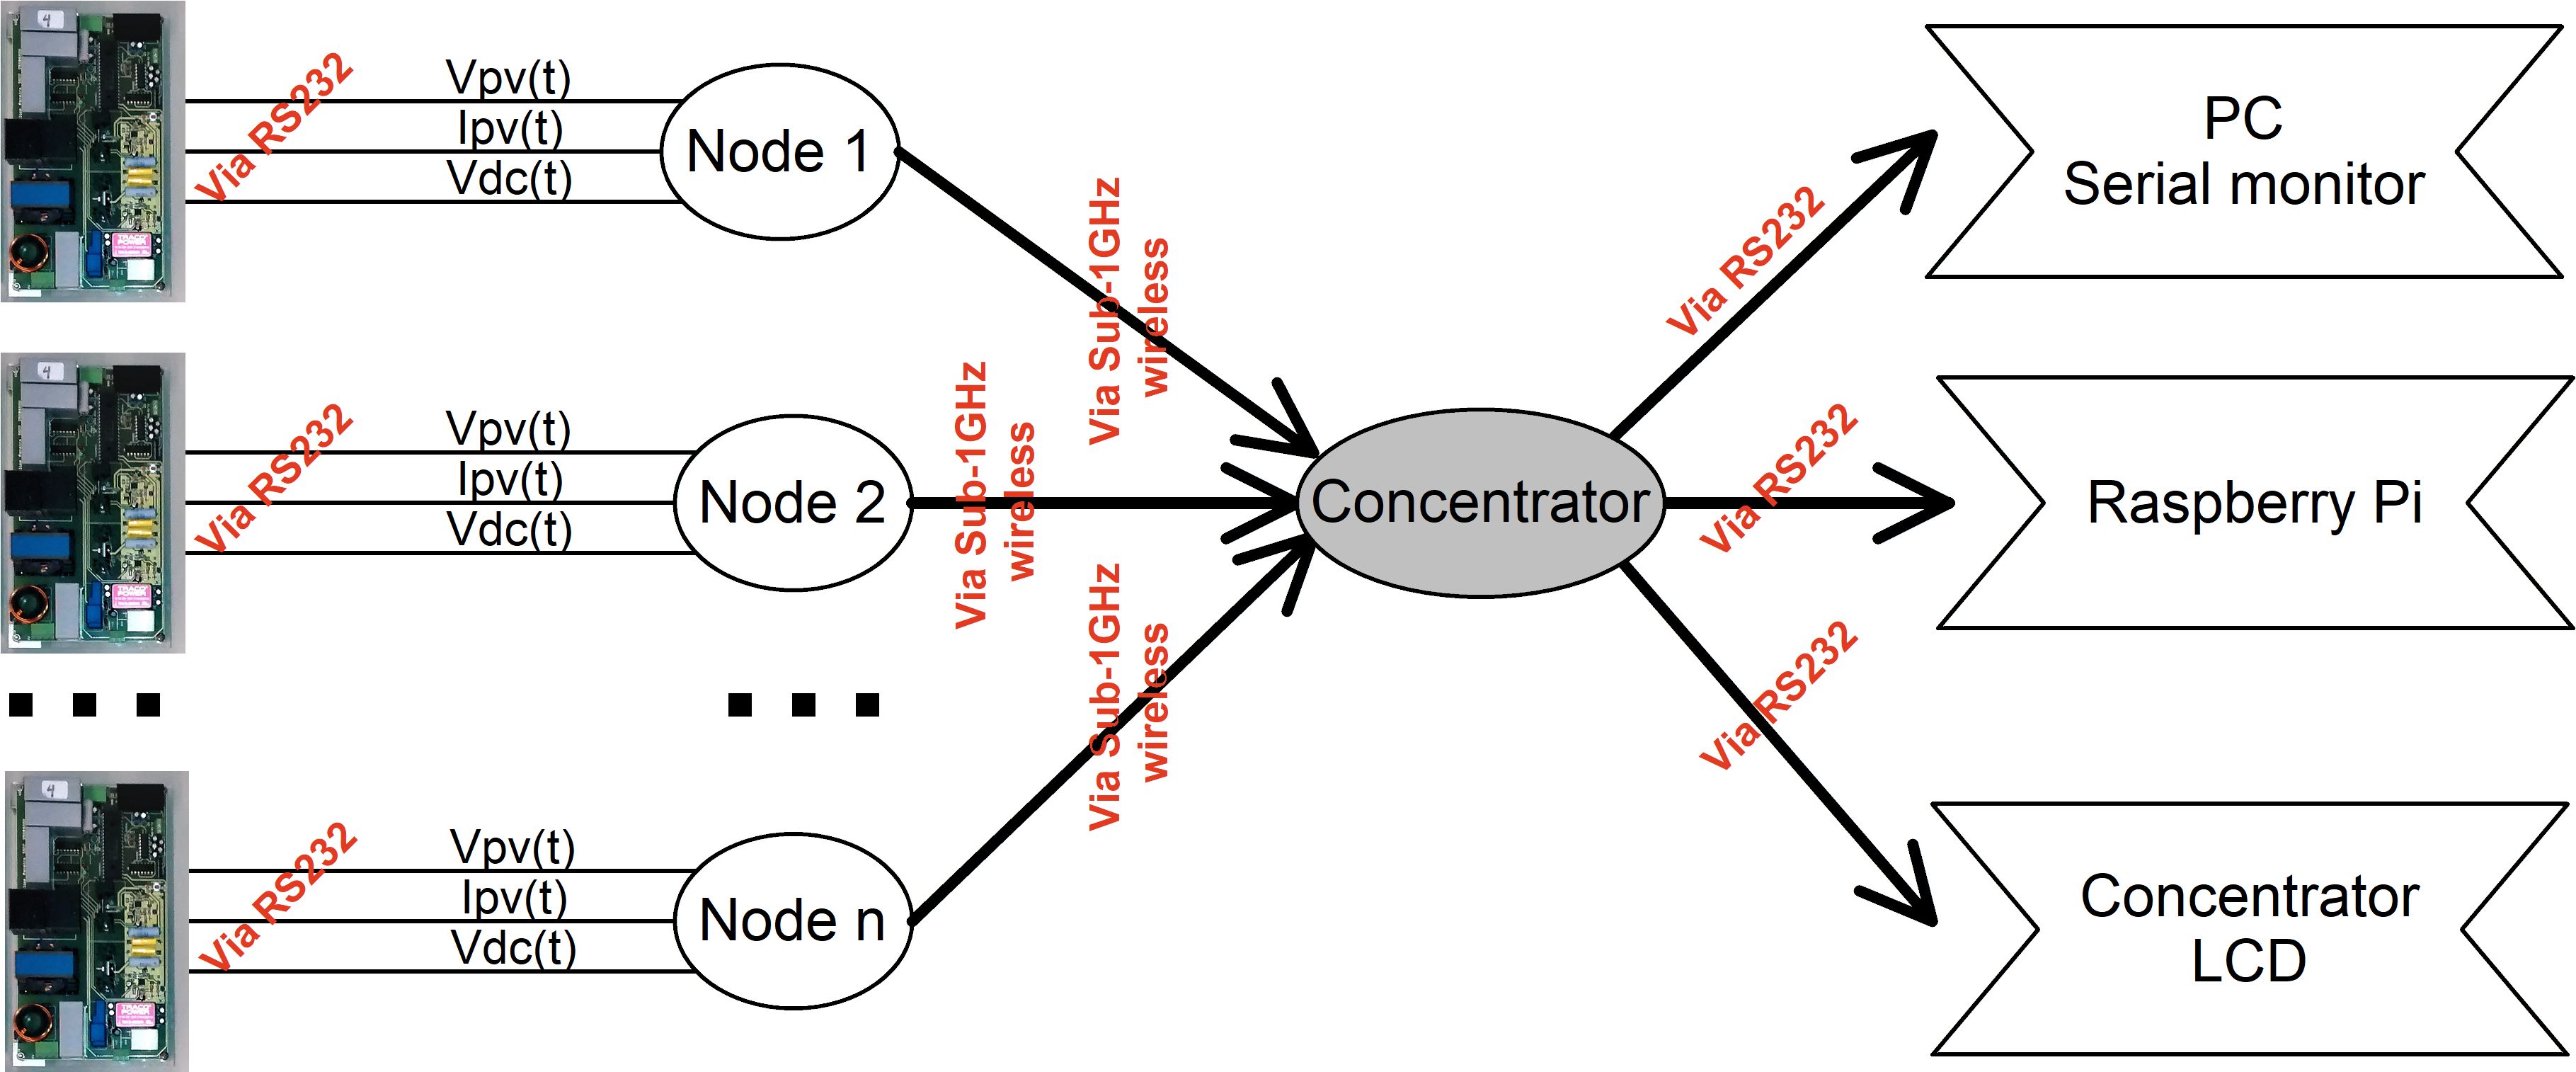
\includegraphics[width=0.9\textwidth,keepaspectratio]{figures/hw}
	\caption{Hardware architecture.}
	\label{fig:3.2.hw}
\end{figure}


\section{Communication results and KPI metrics}
\label{sec:3.3}
\lipsum[4-4]

\section{Discussion of the results}
\label{sec:3.4}
\lipsum[4-4]